\newpage
\def\thoigian{90}%--Thời gian
\de{Đề số 3}{Chương VI. Xác suất}



\begin{center}
	\textbf{PHẦN 1 - CÂU TRẮC NGHIỆM BỐN PHƯƠNG ÁN}
\end{center}
\Opensolutionfile{ans}[ans/ans-TN-ONTAPCHUONG6-DE3]
%Câu 1- Xác suất có điều kiện
\begin{ex}%[2D6H1-2]%[Dự án D - đợt 4 NH24-25- Hieu Hieu Minh Minh]
	Một hộp chứa $5$ quả bóng $2$ quả màu đỏ (đánh số $1$ và $2$), $2$ quả màu xanh (đánh số $3$ và $4$) và $1$ quả màu vàng (đánh số $5$). Lấy ngẫu nhiên $2$ quả bóng liên tiếp không hoàn lại. \\
	Xét các biến cố:\\
	$A\colon$ \lq\lq Quả bóng lấy ra đầu tiên có màu đỏ \rq\rq.\\
	$B\colon$ \lq\lq Tổng số của hai quả bóng lấy ra là số lẻ\rq\rq.\\
	Xác định $B|A$ là biến cố $B$ khi biết $A$ đã xảy ra.
	\choice
	{\True $B|A=\left\{ \left( 1,2 \right);\left( 1,4 \right);\left( 2,1 \right);\left( 2,3 \right);\left( 2,5 \right)\right\}$}
	{$B|A=\left\{ \left( 1,2 \right);\left( 1,4 \right);\left( 2,1 \right);\left( 2,3 \right) \right\}$}
	{$B|A=\left\{ \left( 1,3 \right);\left( 1,5 \right);\left( 2,3 \right);\left( 2,5 \right) \right\}$}
	{$B|A=\left\{ \left( 1,3 \right);\left( 1,5 \right);\left( 2,1 \right);\left( 2,3 \right);\left( 2,5 \right) \right\}$}
	\loigiai{
		Khi $A$ đã xảy ra, nghĩa là quả bóng đầu tiên lấy ra có màu đỏ (số $1$ hoặc $2$). Do đó, không gian mẫu mới là ${\Omega }'=A=\left\{ \left( 1,2 \right);\left( 1,3 \right);\left( 1,4 \right);\left( 1,5 \right);\left( 2,1 \right);\left( 2,3 \right);\left( 2,4 \right);\left( 2,5 \right) \right\}$.\\
		Biến cố $B$ khi biết $A$ đã xảy ra là $B|A=A\cap B=\left\{ \left( 1,2 \right);\left( 1,4 \right);\left( 2,1 \right);\left( 2,3 \right);\left( 2,5 \right) \right\}$.
	}
\end{ex}

%Câu 2 - Xác suất có điều kiện
\begin{ex}%[2D6H1-2]%[Dự án D - đợt 4 NH24-25- Hieu Hieu Minh Minh]
	Cho hai biến cố $A$ và $B$ có $\mathrm{P}(A) = 0{,}76$, $\mathrm{P}(B) = 0{,}28$, $\mathrm{P}(A\,|\,B) = 0{,}50$. Tính xác suất $\mathrm{P}(A\overline{B})$.
	\choice
	{$0{,}14$}
	{\True $0{,}62$}
	{$0{,}38$}
	{$0{,}11$}
	\loigiai{
		$\mathrm{P}(AB) = \mathrm{P}(A\,|\,B)\cdot \mathrm{P}(B) = 0{,}5\cdot 0{,}28 = 0{,}14$.\\
		Vậy $\mathrm{P}(A\overline{B}) = \mathrm{P}(A) - \mathrm{P}(AB) = 0{,}76 - 0{,}14 = 0{,}62$.
	}
\end{ex}
%Câu 3 - Xác suất có điều kiện
\begin{ex}%[2D6H1-2]%[Dự án D - đợt 4 NH24-25- Hieu Hieu Minh Minh]
	Trong cuộc khảo sát trên một nhóm học sinh gồm các bạn thích trà sữa hoặc kem, người ta có được kết quả sau: Có $68\%$ số học sinh thích kem, $56\%$ số học sinh thích trà sữa, $24\%$ số học sinh thích cả trà sữa và kem. Chọn ngẫu nhiên một bạn học sinh trong nhóm được khảo sát này. Tính xác suất để chọn được học sinh thích kem, biết rằng học sinh đó thích trà sữa (làm tròn kết quả đến hàng phần trăm).
	\choice
	{$0{,}42$}
	{$0{,}38$}
	{\True $0{,}43$}
	{$0{,}35$}
	\loigiai{
		Ta gọi các biến cố sau
		\begin{itemize}
			\item Biến cố $K\colon$\lq \lq Học sinh được chọn thích kem\rq \rq, suy ra $\mathrm{P}(K) = 0{,}68$.
			\item Biến cố $T\colon$\lq \lq Học sinh được chọn thích trà sữa\rq \rq, suy ra $\mathrm{P}(T) = 0{,}56$.
		\end{itemize}
		Do đó $\mathrm{P}(KT) = 0{,}24$.\\
		Vậy $\mathrm{P}(K\,|\,T) = \dfrac{\mathrm{P}(KT)}{\mathrm{P}(T)} = \dfrac{0{,}24}{0{,}56} \approx 0{,}4286 \approx 0{,}43$.
	}
\end{ex}
%Câu 4 - Xác suất có điều kiện
\begin{ex}%[2D5N1-1]%[Dự án D - đợt 4 NH24-25- Hieu Hieu Minh Minh]
	Cho hai biến cố $A$, $B$ với $\mathrm{P}(AB)=0{,}2$, $\mathrm{P}(B)=0{,}5$. Khi đó, $\mathrm{P}(A|B)$ bằng
	\choice
	{$0{,}3$}
	{$0{,}2$}
	{\True $0{,}4$}
	{$0{,}8$}
	\loigiai{
		Xác suất có điều kiện được tính theo công thức $
		\mathrm{P}(A|B) = \dfrac{\mathrm{P}(AB)}{P(B)} = \dfrac{0{,}2}{0{,}5} = 0{,}4$. 
	}
\end{ex}
%Câu 5 - Xác suất có điều kiện
\begin{ex}%[2D6H1-2]%[Dự án D - đợt 4 NH24-25- Hieu Hieu Minh Minh]
	Cho hai biến cố $A$ và $B$ là hai biến cố độc lập, với $P\left( A \right)=0{,}2024$, $P\left( B \right)=0{,}2025$. Tính $P\left( B|\overline{A} \right)$.
	\choice
	{$0{,}7976$}
	{$0{,}7975$}
	{\True $0{,}2025$}
	{$0{,}2024$}
	\loigiai{
		$\overline{A}$ và $B$ là hai biến cố độc lập nên $P\left( B|\overline{A} \right)=P\left( B \right)=0{,}2025$.
	}
\end{ex}
%Câu 6 - Xác suất có điều kiện
\begin{ex}%[2D6H1-2]%[Dự án D - đợt 4 NH24-25- Hieu Hieu Minh Minh]
	Cho hai biến cố $A$ và $B$, với $P\left( A \right)=0{,}8$; $P\left( B \right)=0{,}65$ và $P\left( A\cap \overline{B} \right)=0{,}55$. Tính $P\left( A\cap B \right)$.
	\choice
	{\True $0{,}25$}
	{$0{,}1$}
	{$0{,}15$}
	{$0{,}35$}
	\loigiai{
		Ta có $P\left( A\cap \overline{B} \right)+P\left( A\cap B \right)=P\left( A \right)\Rightarrow P\left( A\cap B \right)=P\left( A \right)-P\left( A\cap \overline{B} \right)=0{,}8-0{,}55=0{,}25$.
	}
\end{ex}
%Câu 7 - Xác suất toàn phần và công thức Bayes
\begin{ex}%[2D6N2-1]%[Dự án D - đợt 4 NH24-25- Hieu Hieu Minh Minh]
	Cho $A$, $B$ là các biến cố của một phép thử $T.$ Biết rằng $P\left( A \right)>0$ và $0< P\left( B \right)< 1.$ Xác suất của biến cố $B$ với điều kiện biến cố $A$ đã xảy ra được tính theo công thức nào sau đây?
	\choice
	{$P\left( \left. B \right|A \right)=\dfrac{P\left( A \right) \cdot P\left( \left. A \right|B \right)}{P\left( B \right) \cdot P\left( \left. A \right|B \right)+P\left( {\overline{B}} \right) \cdot P\left( \left. A \right|\overline{B} \right)}$}
	{$P\left( \left. B \right|A \right)=\dfrac{P\left( B \right) \cdot P\left( \left. A \right|B 	\right)}{P\left( A \right) \cdot P\left( \left. B \right|A \right)+P\left( {\overline{A}} \right) \cdot P\left( \left. B \right|\overline{A} \right)}$}
	{\True $P\left( \left. B \right|A \right)=\dfrac{P\left( B \right) \cdot P\left( \left. A \right|B \right)}{P\left( B \right) \cdot P\left( \left. A \right|B \right)+P\left( {\overline{B}} \right) \cdot P\left( \left. A \right|\overline{B} \right)}$}
	{$P\left( \left. B \right|A \right)=\dfrac{P\left( A \right) \cdot P\left( \left. A \right|B \right)}{P\left( A \right) \cdot P\left( \left. B \right|A \right)+P\left( \left. B \right|\overline{A} \right)}$}
	\loigiai{
		Theo công thức Bayes, ta có $P\left( \left. B \right|A \right)=\dfrac{P\left( B \right) \cdot P\left( \left. A \right|B \right)}{P\left( B \right) \cdot P\left( \left. A \right|B \right)+P\left( {\overline{B}} \right) \cdot P\left( \left. A \right|\overline{B} \right)}.$
		
	}
\end{ex}
%Câu 8 - Xác suất toàn phần và công thức Bayes
\begin{ex}%[2D6H2-2]%[Dự án D - đợt 4 NH24-25- Hieu Hieu Minh Minh]
	Cho hai biến cố $A$, $B$ với $P\left( B \right)=0{,}6$; $P\left( A\mid B \right)=0{,}7$ và $P\left( A\mid \overline{B} \right)=0{,}4$. Khi đó, $P\left( A \right)$ bằng
	\choice
	{$0{,}7$}
	{$0{,}4$}
	{\True $0{,}58$}
	{$0{,}52$}
	\loigiai{
		Ta có $P\left( {\overline{B}} \right)=1-P\left( B \right)=1-0{,}6=0{,}4$.\\
		Theo công thức xác suất toàn phần, ta có\\
		$P\left( A \right)=P\left( B \right) \cdot P\left( A\mid B \right)+P\left( {\overline{B}} \right) \cdot P\left( A\mid \overline{B} \right)=0{,}6\cdot 0{,}7+0{,}4 \cdot 0{,}4=0{,}58$.
	}
\end{ex}
%Câu 9 - Xác suất toàn phần và công thức Bayes
\begin{ex}%[2D6H2-2]%[Dự án D - đợt 4 NH24-25- Hieu Hieu Minh Minh]
	Một cửa hàng bán bóng đèn nhập khẩu từ hai nhà máy. Nhà máy $A$ cung cấp $70\%$ tổng số bóng đèn, với tỷ lệ bóng đèn bị lỗi là $2\%$. Nhà máy $B$ cung cấp $30\%$ tổng số bóng đèn, với tỷ lệ bóng đèn bị lỗi là $4\%$. Xác suất để một bóng đèn bất kỳ được chọn ngẫu nhiên từ lô hàng của cửa hàng bị lỗi là
	\choice
	{$0{,}04$}
	{\True $0{,}026$}
	{$0{,}02$}
	{$0{,}06$}
	\loigiai{ 
		\begin{itemize}
			\item Gọi biến cố $A\colon$\lq\lq Bóng đèn được chọn đến từ nhà máy $A$\rq\rq.
			\item Gọi biến cố $B\colon$\lq\lq Bóng đèn được chọn bị lỗi\rq\rq. 
		\end{itemize}
		Ta có $\mathrm{P}(A)=0{,}7$, $\mathrm{P}(B|A)=0{,}02$, $\mathrm{P}\left(\overline{A}\right)=0{,}3$, $\mathrm{P}\left(B|\overline{A}\right)=0{,}04$.\\
		Khi đó $\mathrm{P}(B)=\mathrm{P}(A)\cdot\mathrm{P}(B|A)+\mathrm{P}\left(\overline{A}\right)\cdot\mathrm{P}\left(B|\overline{A}\right)=0{,}7\cdot0{,}02+0{,}3\cdot0{,}04=0{,}026$.
	}
\end{ex}
%Câu 10 - Xác suất toàn phần và công thức Bayes
\begin{ex}%[2D6H2-2]%[Dự án D - đợt 4 NH24-25- Hieu Hieu Minh Minh]
	Cho hai biến cố $A$ và $B$, với $\mathrm{P}(B)=0{,}8$, $\mathrm{P}(A|B)=0{,}7$, $\mathrm{P}(A\overline{B})=0{,}15$. Tính $\mathrm{P}(A)$.
	\choice
	{$0{,}25$}
	{\True $0{,}71$}
	{$0{,}55$}
	{$0{,}5$}
	\loigiai{Áp dụng công thức xác suất toàn phần, ta có $$\mathrm{P}(A)=\mathrm{P}(AB)+\mathrm{P}(A\overline{B})=\mathrm{P}(A|B)\cdot \mathrm{P}(B)+\mathrm{P}(A\overline{B})=0{,}7\cdot0{,}8+0{,}15=0{,}71.$$}
\end{ex}
%Câu 11 - Xác suất toàn phần và công thức Bayes
\begin{ex}%[2D6N2-1]%[Dự án D - đợt 4 NH24-25- Hieu Hieu Minh Minh]
	Cho hai biến cố $M, N$ với $0 < \mathrm{P}(N) < 1$. Chọn khẳng định đúng trong các khẳng định sau đây
	\choice
	{\True $\mathrm{P}(M) = \mathrm{P}(\overline{N})\cdot\mathrm{P}(M|\overline{N}) + \mathrm{P}(N)\cdot\mathrm{P}(M|N)$}
	{$\mathrm{P}(M) = \mathrm{P}(N)\cdot\mathrm{P}(M|N) - \mathrm{P}(\overline{N})\cdot\mathrm{P}(M|\overline{N})$}
	{$\mathrm{P}(M) = \mathrm{P}(\overline{N})\cdot\mathrm{P}(M|\overline{N}) - \mathrm{P}(N)\cdot\mathrm{P}(M|N)$}
	{$\mathrm{P}(M) = \mathrm{P}(N)\cdot\mathrm{P}(M|N) + \mathrm{P}(\overline{N})\cdot\mathrm{P}(M|\overline{N})$}
	\loigiai{
		Theo công thức xác suất toàn phần, ta có
		$$ \mathrm{P}(M) = \mathrm{P}(M \cap N) + \mathrm{P}(M \cap \overline{N}) $$\\
		Theo công thức nhân xác suất
		\begin{itemize}
			\item $\mathrm{P}(M \cap N) = \mathrm{P}(N) \cdot \mathrm{P}(M|N)$ (vì $\mathrm{P}(N) > 0$ theo giả thiết).
			\item $\mathrm{P}(M \cap \overline{N}) = \mathrm{P}(\overline{N}) \cdot \mathrm{P}(M|\overline{N})$.
		\end{itemize}
		Vì $0 < \mathrm{P}(N) < 1$, nên $\mathrm{P}(\overline{N}) = 1 - \mathrm{P}(N)$ cũng thỏa $0 < \mathrm{P}(\overline{N}) < 1$, do đó $\mathrm{P}(\overline{N}) > 0$.\\
		Thay vào công thức xác suất toàn phần, ta được
		$$ \mathrm{P}(M) = \mathrm{P}(N)\mathrm{P}(M|N) + \mathrm{P}(\overline{N})\mathrm{P}(M|\overline{N}). $$
		Công thức này có thể viết lại thứ tự các số hạng
		$$ \mathrm{P}(M) = \mathrm{P}(\overline{N})\mathrm{P}(M|\overline{N}) + \mathrm{P}(N)\mathrm{P}(M|N). $$
	}
\end{ex}
%Câu 12 - Xác suất toàn phần và công thức Bayes
\begin{ex}%[2D5H2-2]%[Dự án D - đợt 4 NH24-25- Hieu Hieu Minh Minh]
	Giả sử tỉ lệ người dân của một tỉnh nghiện thuốc lá là $20$\%, tỉ lệ người bị bệnh phổi trong số người nghiện thuốc lá là $70$\%, trong số người không nghiện thuốc lá là $15$\%. Hỏi khi ta gặp ngẫu nhiên một người dân của tỉnh đó thì khả năng mà người đó bị bệnh phổi là bao nhiêu phần trăm?
	\choice
	{\True $26$\%}
	{$15$\%}
	{$31$\%}
	{$29$\%}
	\loigiai{
		Gọi biến cố $A\colon$\lq\lq Người được chọn nghiện thuốc lá\rq\rq;\\
		Gọi biến cố $B\colon$\lq\lq Người được chọn bị bệnh phổi\rq\rq.\\
		Theo đề bài, ta có
		\begin{itemize}
			\item $\mathrm{P}(A) = 20\% = 0{,}2$ (xác suất người đó nghiện thuốc lá).
			\item $\mathrm{P}(\overline{A}) = 1 - \mathrm{P}(A) = 1 - 0{,}2 = 0{,}8$ (xác suất người đó không nghiện thuốc lá).
			\item $\mathrm{P}(B\mid A) = 70\% = 0{,}7$ (xác suất người đó bị bệnh phổi nếu người đó nghiện thuốc lá).
			\item $\mathrm{P}(B\mid \overline{A}) = 15\% = 0{,}15$ (xác suất người đó bị bệnh phổi nếu người đó không nghiện thuốc lá).
		\end{itemize}
		Xác suất người được chọn bị bệnh phổi là 
		$$\mathrm{P}(B) = \mathrm{P}(A) \cdot \mathrm{P}(B\mid A) + \mathrm{P}(\overline{A}) \cdot \mathrm{P}(B\mid \overline{A})= 0{,}2 \cdot 0{,}7 + 0{,}8\cdot 0{,}15=0{,}26=26\%.$$
	}
\end{ex}

\Closesolutionfile{ans}
%\begin{center}
%	\textbf{ĐÁP ÁN}
%	\inputansbox{10}{ans/ans}	
%\end{center}

\begin{center}
	\textbf{PHẦN 2 - CÂU TRẮC NGHIỆM ĐÚNG SAI}
\end{center}
\setcounter{ex}{0}
\Opensolutionfile{ans}[ans/answer-DS-ONTAPCHUONG6-DE3]
%Câu 1%
\begin{ex}%[2D5V2-3]%[Dự án D - đợt 4 NH24-25- Hieu Hieu Minh Minh]
	Khi kiểm tra sức khoẻ tổng quát của bệnh nhân ở một bệnh viện $A$, người ta được kết quả như sau
	\begin{itemize}
		\item Có $40\%$ bệnh nhân bị đau dạ dày.
		\item Có $30\%$ bệnh nhân thường xuyên bị stress.
		\item Trong số các bệnh nhân bị stress có $80\%$ bệnh nhân bị đau dạ dày.
	\end{itemize}	
	Chọn ngẫu nhiên $1$ bệnh nhân.
	\choiceTF
	{\True Xác suất chọn được bệnh nhân thường xuyên bị stress là $0{,}3$}
	{Xác suất chọn được bệnh nhân bị đau dạ dày, biết bệnh nhân đó thường xuyên bị stress là $0{,}7$}
	{\True Xác suất chọn được bệnh nhân vừa thường xuyên bị stress vừa bị đau dạ dày là $0{,}24$}
	{\True Xác suất chọn được bệnh nhân thường xuyên bị stress, biết bệnh nhân đó bị đau dạ dày là $0{,}6$}
	\loigiai{
		Gọi biến cố $A\colon$ \lq\lq Bệnh nhân thường xuyên bị stress\rq\rq\  và $B\colon$ \lq\lq Bệnh nhân bị đau dạ dày\rq\rq.\\
		Khi đó $P(B)=0{,}4$.
		\begin{center}
			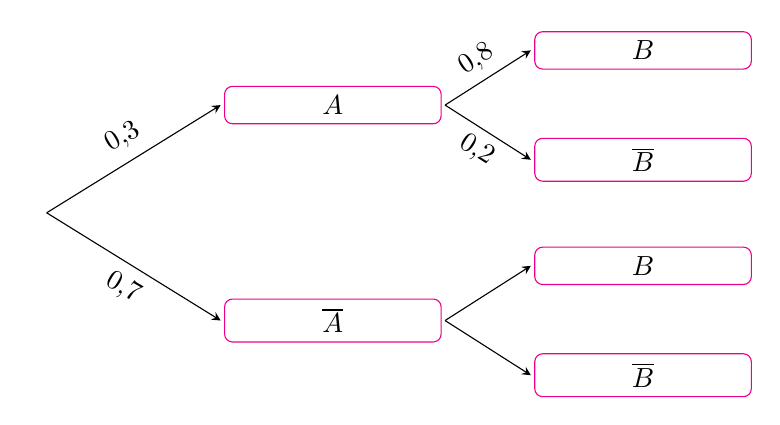
\begin{tikzpicture}
				\def\gocm{20}
				\def\gocn{10}
				\def\r{4}
				\tikzset{s/.style={outer sep=0.5 mm,draw=magenta,rectangle,minimum width=2.75cm,rounded corners=1mm}}
				\path(0,0)node(O){}++(\gocm:\r)node[s](A1){$A$}++(\gocn:\r)node[s](A2){$B$};
				\path(A1)++({-\gocn}:\r)node[s](a2){$\overline{B}$};
				\path(O)++(-\gocm:\r)node[s](B1){$\overline{A}$}++(\gocn:\r)node[s](B2){$B$};
				\path(B1)++({-\gocn}:\r)node[s](b2){$\overline{B}$};
				\foreach \x/\y in {
					O/A1,A1/A2,
					O/B1,B1/B2,
					A1/a2,
					B1/b2}
				\draw[-stealth](\x.east)--(\y.west);
				\path(O)--(A1.west)node[pos=0.5,above,sloped]{$\mbox{0{,}3}$}(O)--(B1.west)node[pos=0.5,below,sloped]{$\mbox{0{,}7}$}(B1.east)--(B2.west)node[pos=0.5,above,sloped]{$\mbox{}$}(A1.east)--(A2.west)node[pos=0.5,above,sloped]{$\mbox{0{,}8}$}
				(A1.east)--(a2.west)node[pos=0.5,below,sloped]{$\mbox{0{,}2}$}
				(B1.east)--(b2.west)node[pos=0.5,below,sloped]{$\mbox{ }$};
			\end{tikzpicture}
		\end{center}
		\begin{itemchoice}
			\itemch 
			Xác suất chọn được bệnh nhân thường xuyên bị stress là $0{,}3$.
			\itemch 
			Xác suất chọn được bệnh nhân bị đau dạ dày, biết bệnh nhân đó thường xuyên bị stress là $P(B\mid A)=0{,}8$.
			\itemch 
			Xác suất chọn được bệnh nhân vừa thường xuyên bị stress vừa bị đau dạ dày là $P(AB)=0{,}3\cdot 0{,}8=0{,}24$.
			\itemch 
			$P(A\mid B)=\dfrac{P(A)\cdot P(B\mid A)}{P(B)}=\dfrac{0{,}3\cdot 0{,}8}{0{,}4}=0{,}6$.
		\end{itemchoice}
	}
\end{ex}
%Câu 2%
\begin{ex}%[2D6H2-4]%[Dự án D - đợt 4 NH24-25- Hieu Hieu Minh Minh]
	Một cửa hàng có hai máy sản xuất bánh ngọt. Máy thứ nhất sản xuất $70\%$ tổng số bánh của cửa hàng. Tỉ lệ bánh bị cháy của máy thứ nhất và máy thứ hai lần lượt là $5\%$ và $8\%$. Lấy ngẫu nhiên một chiếc bánh trong lô hàng của cửa hàng. Gọi $A$ là biến cố \lq\lq Chiếc bánh được sản xuất từ nhà máy thứ nhất\rq\rq\, và $B$ là biến cố \lq\lq Chiếc bánh bị cháy\rq\rq.
	\choiceTF
	{\True $\mathrm{P}(A)=0{,}7$ và $\mathrm{P}\left(\overline{A}\right)=0{,}3$}
	{\True Xác suất để lấy được bánh bị cháy là $0{,}059$}
	{\True Nếu đã lấy được bánh bị cháy, xác suất bánh đó do máy thứ nhất sản xuất là $0{,}59$ (kết quả được làm tròn đến hàng phầm trăm)}
	{Nếu lấy được bánh không bị cháy, tỉ lệ bánh đó do máy hai sản xuất là $30\%$ (kết quả tính theo phần trăm được làm tròn đến hàng đơn vị)}
	\loigiai{
		\begin{itemchoice}
			\itemch Ta có $\mathrm{P}(A)=0{,}7$ và $\mathrm{P}\left(\overline{A}\right)=0{,}3$.
			\itemch Xác suất lấy được bánh bị cháy là $$\mathrm{P}(B)=\mathrm{P}(A)\cdot \mathrm{P}(B\mid A)+\mathrm{P}\left(\overline{A}\right)\cdot \mathrm{P}\left(B\mid\overline{A}\right)=0{,}7\cdot{,}05+0{,}3\cdot 0{,}08=0{,}059.$$
			\itemch Ta có $\mathrm{P}(A\mid B)=\dfrac{\mathrm{P}(A)\cdot\mathrm{P}(B|A)}{\mathrm{P}(B)}=\dfrac{0{,}7\cdot0{,}05}{0{,}059}\approx 0{,}59$.
			\itemch Ta có $\mathrm{P}\left(\overline{A}\mid \overline{B}\right)=\dfrac{\mathrm{P}\left(\overline{A}\right)\cdot\mathrm{P}\left(\overline{B}\mid \overline{A}\right)}{\mathrm{P}\left(\overline{B}\right)}=\dfrac{0{,}3\cdot0{,}08}{1-0{,}059}\approx 0{,}03=3\%$.
		\end{itemchoice}
	}
\end{ex}

\Closesolutionfile{ans}
%\inputansbox[2]{2}{ans/answer.tex}

\begin{center}
\textbf{PHẦN 3 - CÂU TRẮC NGHIỆM TRẢ LỜI NGẮN}
\end{center}
\setcounter{ex}{0}
\Opensolutionfile{ans}[ans/ans-KQ-ONTAPCHUONG6-DE3]
%Câu 1%
\begin{ex}%[2D6H1-2]%[Dự án D - đợt 4 NH24-25- Hieu Hieu Minh Minh]
	Khảo sát một nhóm $100$ người dùng mạng xã hội, người ta thống kê được rằng $60$ người sử dụng Facebook, $45$ người sử dụng TikTok và $25$ người sử dụng cả Facebook và TikTok. Chọn ngẫu nhiên một người từ nhóm này. Xác suất để người đó sử dụng TikTok là bao nhiêu, biết rằng người đó đã sử dụng Facebook? (kết quả làm tròn đến hàng phần trăm)
	\shortans{$0{,}42$}
	\loigiai{
		Gọi $A$ là biến cố \lq\lq người được chọn sử dụng Facebook\rq\rq.\\
		Gọi $B$ là biến cố \lq\lq người được chọn sử dụng TikTok\rq\rq.\\
		Ta có $n(A) = 60$,	$n(B) = 45$ và $n(A \cap B) = 25$.\\
		Xác suất để người đó sử dụng TikTok biết rằng người đó đã sử dụng Facebook là 
		$$\mathrm{P}(B|A)= \dfrac{n(A \cap B)}{n(A)} = \dfrac{25}{60} \approx 0{,}42.$$
	}
\end{ex}
%Câu 2%
\begin{ex}%[2D6H1-2]%[Dự án D - đợt 4 NH24-25- Hieu Hieu Minh Minh]
	Bạn An phải thực hiện hai thí nghiệm liên tiếp. Thí nghiệm thứ nhất có xác suất thành công là $0{,}7$. Nếu thí nghiệm thứ nhất thành công thì xác suất thành công của thí nghiệm thứ hai là $0{,}9$. Tính xác suất để thí nghiệm thứ nhất thành công và thí nghiệm thứ hai không thành công.
	\shortans[oly]{0,07}
	\loigiai{
		Gọi biến cố $A\colon$\lq\lq Thí nghiệm thứ nhất thành công\rq\rq. Ta có $\mathrm{P}(A)=0{,}7$.\\
		Gọi biến cố $B\colon$\lq\lq Thí nghiệm thứ hai thành công\rq\rq.\\
		Xác suất thí nghiệm thứ hai thành công nếu thí nghiệm thứ nhất đã thành công là \[\mathrm{P}(B|A)=0{,}9.\]	
		Xác suất để thí nghiệm thứ hai không thành công, với điều kiện thí nghiệm thứ nhất đã thành công là
		\[\mathrm{P}(\overline{B}|A)=1-\mathrm{P}(B|A)=1-0{,}9=0{,}1. \]
		Vậy xác suất để thí nghiệm thứ nhất thành công và thí nghiệm thứ hai không thành công là
		\[\mathrm{P}(A \cap \overline{B})=\mathrm{P}(A) \cdot \mathrm{P}(\overline{B}|A)=0{,}7 \cdot 0{,}1=0{,}07. \]
	}
\end{ex}
%Câu 3%
\begin{ex}%[2D6V2-2]%[Dự án D - đợt 4 NH24-25- Hieu Hieu Minh Minh]
	Một trường THPT mới thành lập có hai khối $10$ và $11$. Biết tỉ lệ học sinh khối $10$ và khối $11$ là $7:8$. Tỉ lệ học sinh đạt danh hiệu học sinh khá trở lên của trường là $65\%$ và tỉ lệ này ở khối $11$ là $70\%$. Chọn ngẫu nhiên một học sinh của trường. Tính xác suất học sinh được chọn đạt danh hiệu học sinh khá trở lên của khối $10$. (kết quả làm tròn đến hàng phần trăm)
	\shortans{$0{,}59$}
	\loigiai{
		Gọi $K_{10}$ là biến cố \lq\lq học sinh được chọn thuộc khối $10$\rq\rq.\\
		Gọi $K_{11}$ là biến cố \lq\lq học sinh được chọn thuộc khối $11$\rq\rq.\\
		Gọi $H$ là biến cố \lq\lq học sinh được chọn đạt danh hiệu học sinh khá trở lên\rq\rq.\\
		Tỉ lệ học sinh khối $10$ và khối $11$ là $7:8$, tức là\\
		$\mathrm{P}(K_{10}) = \dfrac{7}{7+8} = \dfrac{7}{15}$ và $\mathrm{P}(K_{11}) = \dfrac{8}{7+8} = \dfrac{8}{15}$.\\
		Tỉ lệ học sinh đạt danh hiệu học sinh khá trở lên của trường là $65\%$, tức là $\mathrm{P}(H) = 0{,}65$.\\
		Tỉ lệ học sinh đạt danh hiệu học sinh khá trở lên ở khối $11$ là $70\%$, tức là $\mathrm{P}(H|K_{11}) = 0{,}7$.\\
		Ta cần tính $\mathrm{P}(H|K_{10})$.\\
		Áp dụng công thức xác suất toàn phần: 
		\begin{eqnarray*}
			&&\mathrm{P}(H) = \mathrm{P}(H|K_{10})\mathrm{P}(K_{10}) + \mathrm{P}(H|K_{11})\mathrm{P}(K_{11})\\
			&\Rightarrow& 0{,}65 = \mathrm{P}(H|K_{10}) \cdot \dfrac{7}{15} + 0{,}7 \cdot \dfrac{8}{15}\\
			&\Rightarrow&  \mathrm{P}(H|K_{10}) = \dfrac{83}{140} \approx 0{,}59.
		\end{eqnarray*}
	}
\end{ex}
%Câu 4%
\begin{ex}%[2D6V2-3]%[Dự án D - đợt 4 NH24-25- Hieu Hieu Minh Minh]
	Một nhà máy sản xuất bóng đèn có tỉ lệ bóng đèn đạt tiêu chuẩn là $80$\%. Trước khi xuất ra thị trường, mỗi bóng đèn đều được kiểm tra chất lượng. Vì sự kiểm tra không thể tuyệt đối hoàn hảo nên tỉ lệ công nhận một bóng đèn đạt tiêu chuẩn là $0{,}9$ và tỉ lệ loại bỏ một bóng hỏng là $0{,}95$. Hãy tính tỉ lệ phần trăm bóng đạt tiêu chuẩn sau khi qua khâu kiểm tra chất lượng (làm tròn kết quả đến hàng phần chục).
	\shortans{$98{,}6$}
	\loigiai{
		Gọi $A$ là các biến cố \lq\lq Chọn được bóng đèn đạt tiêu chuẩn\rq\rq.\\
		$B$ là biến cố \lq\lq Chọn được bóng đèn được công nhận là bóng đèn đạt tiêu chuẩn\rq\rq.\\
		Khi đó\\
		Biến cố $\overline{A} \colon$ \lq\lq Chọn được bóng đèn bị hỏng\rq\rq.\\
		Biến cố $\overline{B} \colon$ \lq\lq Chọn được bóng đèn được bị loại bỏ\rq\rq.\\
		Theo giả thiết ta có, $\mathrm{P}(A)=0{,}8$, $\mathrm{P}(B \mid A)=0{,}9$, $\mathrm{P}(\overline{B} \mid \overline{A})=0{,}95$.\\
		Suy ra $\mathrm{P}(\overline{A})=1-\mathrm{P}(A)=0{,}2$ và $\mathrm{P}(B\mid \overline{A})=1-\mathrm{P}(\overline{B} \mid \overline{A})=0{,}05$.\\
		Theo công thức xác suất toàn phần ta có\\
		$\mathrm{P}(B)=\mathrm{P}(A)\mathrm{P}(B \mid A)+\mathrm{P}(\overline{A})\mathrm{P}(B \mid \overline{A})=0{,}8 \cdot 0{,}9+0{,}2\cdot 0{,}05=0{,}73$.\\
		Ta cần tính tỉ lệ bóng đền đạt tiêu chuẩn sau khi kiểm tra, tức là cần tính $\mathrm{P}(A \mid B)$.\\
		Theo công thức Bayes, ta có\\
		$\mathrm{P}(A \mid B)=\dfrac{\mathrm{P}(A)\cdot \mathrm{P}(B \mid A) }{\mathrm{P}(B)}=\dfrac{0{,}8\cdot 0{,}9}{0{,}73}=0{,}98630137$.\\
		Vậy tỉ lệ bóng đạt tiêu chuẩn sau khi qua khâu kiểm tra là $98{,}6$\%.
	}
\end{ex}

\Closesolutionfile{ans}
\begin{center}
	\textbf{PHẦN 4 - TỰ LUẬN}
\end{center}
\setcounter{ex}{0}
%Câu 1%
\begin{ex}%[2D6V1-3]%[Dự án D - đợt 4 NH24-25- Hieu Hieu Minh Minh]
	Một bình đựng $10$ viên bi với kích thước, chất liệu như nhau; trong đó có $6$ viên bi xanh và $4$ viên bi trắng. Lấy ngẫu nhiên ra một viên bi, không hoàn lại, rồi lại lấy ngẫu nhiên ra một viên bi nữa. Tính xác suất để lấy được một viên bi xanh ở lần thứ nhất và một viên bi trắng ở lần thứ hai.
	\loigiai{
		Gọi biến cố $A\colon$ \lq\lq Lấy được viên bi xanh ở lần thứ nhất\rq\rq;\\
		Gọi biến cố $B\colon$ \lq\lq Lấy được viên bi trắng ở lần thứ hai\rq\rq.
		\begin{center}
			\begin{tikzpicture}
				\def\gocm{20}
				\def\gocn{10}
				\def\r{3}
				\tikzset{s/.style={outer sep=0.5 mm,draw=magenta,rectangle,minimum width=1.5cm,rounded corners=1mm}}
				\path
				(0,0)node(O){}++(\gocm:\r)node[s](A1){$A$}++(\gocn:\r)node[s](A2){$B$};
				\path(A1)++({-\gocn}:\r)node[s](a2){$\overline{B}$};
				\path(O)++(-\gocm:\r)node[s](B1){$\overline{A}$}++(\gocn:\r)node[s](B2){$B$};
				\path(B1)++({-\gocn}:\r)node[s](b2){$\overline{B}$};
				\foreach \x/\y in {
					O/A1,A1/A2,
					O/B1,B1/B2,
					A1/a2,
					B1/b2}
				\draw[-stealth](\x.east)--(\y.west);
				\path(O)--(A1.west)node[pos=0.5,above,sloped]{$\tfrac{6}{10}$}(O)--(B1.west)node[pos=0.5,below,sloped]{$\tfrac{4}{10}$}(B1.east)--(B2.west)node[pos=0.5,above,sloped]{$\tfrac{6}{9}$}(A1.east)--(A2.west)node[pos=0.5,above,sloped]{$\tfrac{5}{9}$}
				(A1.east)--(a2.west)node[pos=0.5,below,sloped]{$\tfrac{4}{9}$}
				(B1.east)--(b2.west)node[pos=0.5,below,sloped]{$\tfrac{4}{9}$};
			\end{tikzpicture}
		\end{center}
		Ta có $\mathrm{P}\left(A B\right)=\mathrm{P}\left(A\right) \cdot \mathrm{P}\left(B\mid A\right)=\dfrac{6}{10} \cdot \dfrac{4}{9}= \dfrac{4}{15}$.\\
		Vậy xác suất để lấy được một viên bi xanh ở lần thứ nhất và một viên bi trắng ở lần thứ hai là $\dfrac{4}{15}$.
	}
\end{ex}
%Câu 2%
\begin{ex}%[2D5H2-2]%[Dự án D - đợt 4 NH24-25- Hieu Hieu Minh Minh]
	Trong một kì thi tốt nghiệp trung học phổ thông, một tỉnh $X$ có $60\%$ học sinh lựa chọn tổ hợp $D07$ (gồm các môn Toán, Hóa học, Tiếng Anh). Biết rằng, nếu một học sinh lựa chọn tổ hợp $D07$ thì xác suất để học sinh đó đỗ đại học là $0{,}5$; còn nếu một học sinh không lựa chọn tổ hợp $D07$ thì xác suất để học sinh đó đỗ đại học là $0{,}71$. Chọn ngẫu nhiên một học sinh của tỉnh $X$ đã tốt nghiệp trung học phổ thông trong kì thi trên. Tính xác suất  để học sinh đó đỗ đại học.
	\loigiai{Gọi $A$ là biến cố \lq \lq Học sinh đó lựa chọn tổ hợp $D07$ \rq \rq.\\
		Gọi $B$ là biến cố \lq \lq Học sinh đó đỗ đại học \rq \rq.\\
		Theo giả thiết, ta có $\mathrm{P}(A)=60\%$; $\mathrm{P} \left(B \mid A\right)=0{,}5$; $\mathrm{P} \left(B \mid \overline{A}\right)=0{,}71$.\\
		Theo công thức xác suất toàn phần, ta có
		\begin{align*}
			\mathrm{P} (B)&=\mathrm{P} \left(B \mid A\right) \cdot \mathrm{P} (A)+  \mathrm{P} \left(B \mid \overline{A}\right) \cdot \mathrm{P} \left(\overline{A}\right)\\
			&=0{,}5 \cdot 60\% + 0{,}71 \cdot \left(1-60\%\right)\\
			& = \dfrac{73}{125}.
		\end{align*}
		Vậy xác suất để học sinh được chọn đỗ đại học vào khoảng $\dfrac{73}{125}$.}
\end{ex}
%Câu 3%
\begin{ex}%[2D6V2-2]%[Dự án D - đợt 4 NH24-25- Hieu Hieu Minh Minh]
	Một lớp có $70\%$ học sinh là nữ. Tỉ lệ học sinh nữ đạt danh hiệu học sinh giỏi là $35\%$, tỉ lệ học sinh nam đạt danh hiệu học sinh giỏi là $60\%$. Chọn ngẫu nhiên một học sinh của lớp đó. Gọi $A$ là biến cố \lq \lq Học sinh được chọn là nữ\rq\rq và $B$ là biến cố \lq\lq Học sinh được chọn đạt danh hiệu học sinh giỏi\rq \rq.
	\loigiai{
		Vì $\mathrm{P}(A)=0{,}7$ nên $\mathrm{P}(\overline{A})=0{,}3$.\\
		Ta có $\mathrm{P}(B|A)=0{,}35$ và $\mathrm{P}(B|\overline{A})=0{,}6$.\\
		Khi đó $\mathrm{P}(B)=\mathrm{P}(A)\cdot \mathrm{P}(B|A)+\mathrm{P}(\overline{A})\cdot \mathrm{P}(B|\overline{A})=0{,7}\cdot 0{,}35+0{,}3\cdot 0,6=0{,}425$.
	}
\end{ex}
